\documentclass[aspectratio=169,11pt]{beamer}
\usepackage[T1]{fontenc}
\usepackage{lmodern,amsmath,amssymb,mathtools,bm,booktabs,array,graphicx,tikz}
\usetikzlibrary{arrows.meta,positioning,calc,decorations.pathreplacing,patterns}
\definecolor{ink}{HTML}{17344D}\definecolor{accent}{HTML}{087E8B}\definecolor{pale}{HTML}{EDF5F5}\definecolor{gold}{HTML}{AD6B19}
\providecommand{\dd}{\,\mathrm{d}}\providecommand{\R}{\mathbb{R}}
\providecommand{\E}{\mathbb{E}}\providecommand{\Var}{\operatorname{Var}}
\providecommand{\Cov}{\operatorname{Cov}}\providecommand{\diag}{\operatorname{diag}}
\providecommand{\norm}[1]{\left\lVert#1\right\rVert}
\providecommand{\abs}[1]{\left|#1\right|}
\usefonttheme{professionalfonts}
\setbeamercolor{normal text}{fg=black,bg=white}
\setbeamercolor{frametitle}{fg=ink,bg=white}
\setbeamercolor{title}{fg=ink}\setbeamercolor{structure}{fg=accent}
\setbeamercolor{block title}{fg=ink,bg=pale}\setbeamercolor{block body}{fg=black,bg=pale!40}
\setbeamercolor{alerted text}{fg=accent}
\setbeamerfont{frametitle}{size=\Large,series=\bfseries}
\setbeamerfont{title}{size=\LARGE,series=\bfseries}
\setbeamertemplate{navigation symbols}{}
\setbeamersize{text margin left=.7cm,text margin right=.7cm}
\setbeamertemplate{frametitle}{\vspace{.18cm}\insertframetitle\par\vspace{.1cm}{\color{accent}\hrule height .6pt}\vspace{.12cm}}
\newcommand{\notestarget}{notes.pdf}\newcommand{\noteslabel}{Notes}
\setbeamertemplate{footline}{\hspace{.7cm}\color{ink}\scriptsize Scientific Computing in Python\quad\href{\notestarget}{\noteslabel}\hfill\insertframenumber\,/\,\inserttotalframenumber\hspace{.7cm}\vspace{.18cm}}
\setbeamercovered{invisible}
\hypersetup{pdfauthor={Zan Ahmad},pdftitle={NumPy arrays and linear inverse problems},pdfpagemode=UseNone}
\begin{document}
\begin{frame}[plain]\vfill
{\small\color{accent} Scientific Computing in Python \quad Lecture 3}\par\medskip
{\raggedright\hyphenpenalty=10000\exhyphenpenalty=10000\LARGE\bfseries\color{ink} NumPy arrays and linear inverse problems}\par\bigskip
Zan Ahmad\par\smallskip
{\small Winter 2026}\par\vfill\end{frame}
\renewcommand{\notestarget}{notes.pdf\#note-the-observation-matrix}
\begin{frame}[t,fragile,label=slide-the-observation-matrix]{The observation matrix}
\[
y=Ac,\qquad A=\begin{pmatrix}1&0.25\\0.20&1.20\end{pmatrix},\quad c=\begin{pmatrix}c_A\\c_B\end{pmatrix}.
\]
\pause{}
\[
y_1=c_A+0.25c_B,\qquad y_2=0.20c_A+1.20c_B.
\]
\end{frame}
\renewcommand{\notestarget}{notes.pdf\#note-the-observation-matrix}
\begin{frame}[t,fragile,label=slide-matrix-entries-and-units]{Matrix entries and units}
$A_{ij}$ is the response of detector $i$ to one concentration unit of constituent $j$.
\pause{}
\[
[A_{ij}]=\frac{\text{signal}}{\text{concentration}},\qquad [Ac]=\text{signal}.
\]
The row and column meanings are part of the model.
\end{frame}
\renewcommand{\notestarget}{notes.pdf\#note-rows-of-observations}
\begin{frame}[t,fragile,label=slide-rows-of-observations]{Rows of observations}
\[
C\in\R^{n\times2},\quad A\in\R^{2\times2},\quad Y=CA^{\mathsf T}\in\R^{n\times2}.
\]
\pause{}
\[
Y_{ri}=\sum_{j=1}^{2}C_{rj}A_{ij}.
\]
\end{frame}
\renewcommand{\notestarget}{notes.pdf\#note-rows-of-observations}
\begin{frame}[t,fragile,label=slide-array-multiplication]{Array multiplication}
\begin{verbatim}
Y = C @ A.T
\end{verbatim}
\pause{}
\texttt{@} contracts the shared index. Entrywise \texttt{C*A} is a different operation and need not even have compatible shapes.
\end{frame}
\renewcommand{\notestarget}{notes.pdf\#note-solving-the-calibration-equations}
\begin{frame}[t,fragile,label=slide-solving-the-calibration-equations]{Solving the calibration equations}
\[
\det A=1(1.20)-0.25(0.20)=1.15\ne0.
\]
\pause{}
\begin{verbatim}
c_hat = np.linalg.solve(A, y)
residual = A @ c_hat - y
\end{verbatim}
\end{frame}
\renewcommand{\notestarget}{notes.pdf\#note-the-observation-matrix}
\begin{frame}[label=slide-the-calibration-map-figure]{The calibration map}
\centering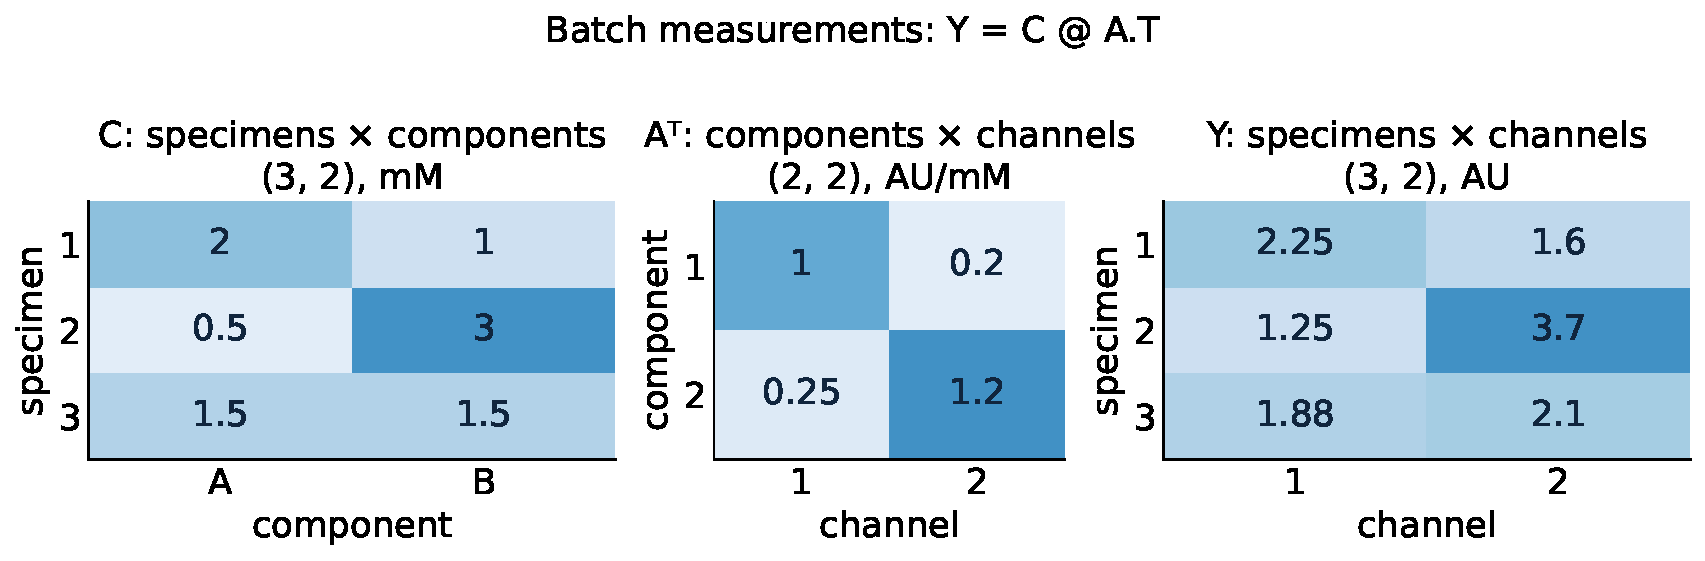
\includegraphics[width=.98\linewidth,height=.69\textheight,keepaspectratio]{presentation-figures/mixture-shapes.pdf}\end{frame}
\renewcommand{\notestarget}{notes.pdf\#note-solving-the-calibration-equations}
\begin{frame}[t,fragile,label=slide-elimination-by-hand]{Elimination by hand}
Subtract $0.20$ times the first detector equation from the second:
\[
1.15c_B=y_2-0.20y_1.
\]
\pause{}
Then $c_A=y_1-0.25c_B$. The numerical solve carries out equivalent linear algebra.
\end{frame}
\renewcommand{\notestarget}{notes.pdf\#note-residual-and-reconstruction-error}
\begin{frame}[t,fragile,label=slide-residual-and-reconstruction-error]{Residual and reconstruction error}
\[
r=A\widehat c-y,\qquad e=\widehat c-c_{\rm true}.
\]
\pause{}
If $y=Ac_{\rm true}+\delta y$ and $r=0$, then
\[
Ae=\delta y.
\]
\end{frame}
\renewcommand{\notestarget}{notes.pdf\#note-residual-and-reconstruction-error}
\begin{frame}[t,fragile,label=slide-a-residual-scaled-to-the-problem]{A residual scaled to the problem}
A dimensionless residual measure is
\[
\eta=\frac{\|A\widehat c-y\|_2}{\|A\|_2\|\widehat c\|_2+\|y\|_2}.
\]
\pause{}
A small $\eta$ supports the algebraic solve. It does not establish accurate calibration or accurate observations. If both numerator and denominator are zero, report the exact zero residual separately.
\end{frame}
\renewcommand{\notestarget}{notes.pdf\#note-conditioning-and-redundant-detectors}
\begin{frame}[t,fragile,label=slide-conditioning-and-redundant-detectors]{Conditioning and redundant detectors}
\[
\delta c=A^{-1}\delta y,
\qquad
\frac{\|\delta c\|_2}{\|c\|_2}\leq\kappa_2(A)\frac{\|\delta y\|_2}{\|y\|_2}.
\]
\pause{}
The bound assumes $A$ is fixed and nonsingular. This relative bound assumes $c\ne0$ and $y\ne0$.
\end{frame}
\renewcommand{\notestarget}{notes.pdf\#note-conditioning-and-redundant-detectors}
\begin{frame}[label=slide-sensitivity-to-detector-noise-figure]{Sensitivity to detector noise}
\centering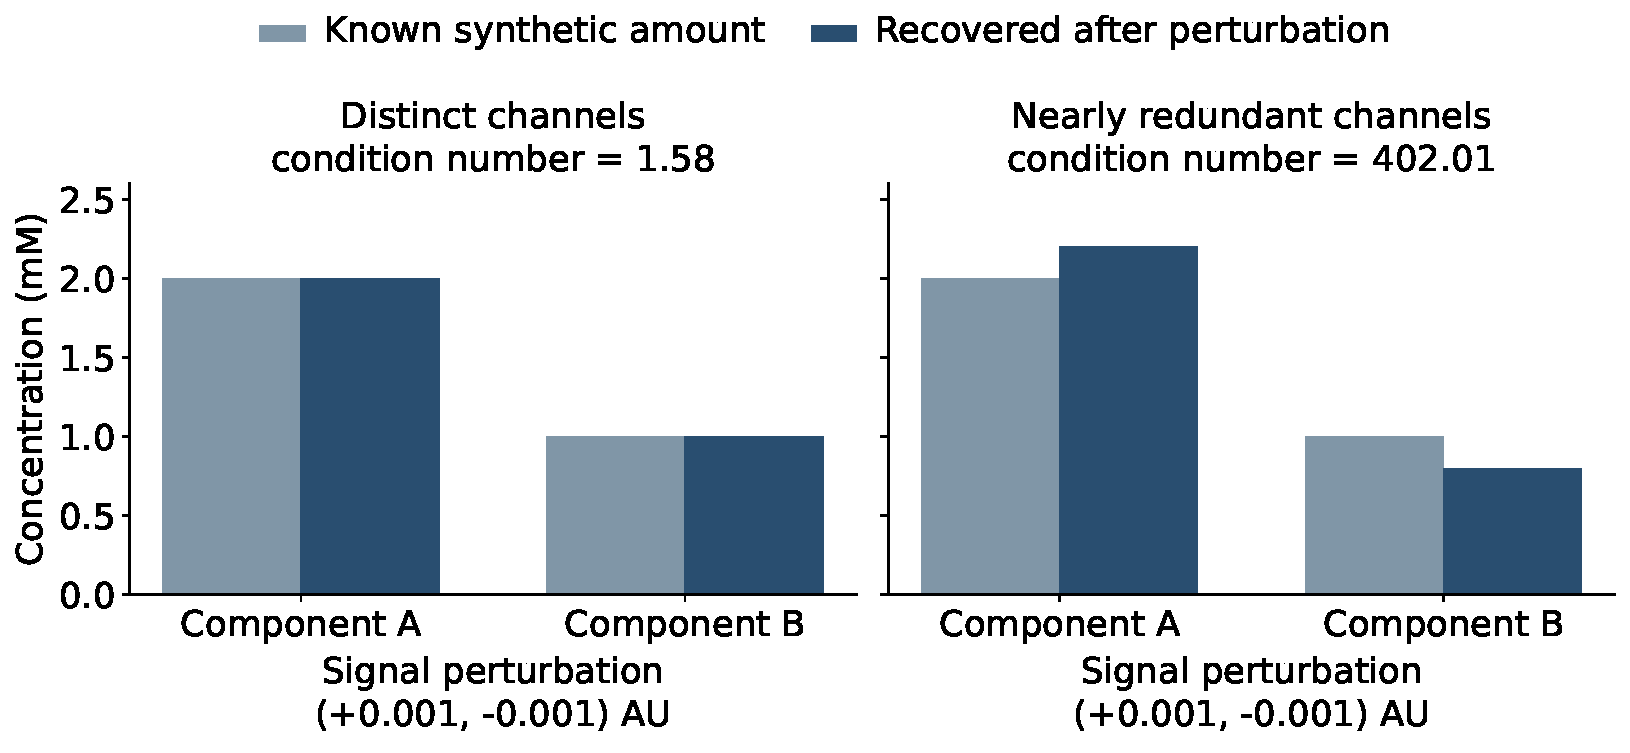
\includegraphics[width=.98\linewidth,height=.69\textheight,keepaspectratio]{presentation-figures/sensitivity.pdf}\end{frame}
\renewcommand{\notestarget}{notes.pdf\#note-conditioning-and-redundant-detectors}
\begin{frame}[t,fragile,label=slide-singular-values]{Singular values}
If $A=U\Sigma V^{\mathsf T}$, then
\[
\kappa_2(A)=\frac{\sigma_{\max}}{\sigma_{\min}}.
\]
\pause{}
A small $\sigma_{\min}$ identifies a concentration direction that produces little signal.
\end{frame}
\renewcommand{\notestarget}{notes.pdf\#note-batch-solves-and-physical-constraints}
\begin{frame}[t,fragile,label=slide-batch-solves-and-physical-constraints]{Batch solves and physical constraints}
\begin{verbatim}
C_hat = np.linalg.solve(A, Y.T).T
\end{verbatim}
\pause{}
This solves the same calibrated map for every row of observations.
\end{frame}
\renewcommand{\notestarget}{notes.pdf\#note-batch-solves-and-physical-constraints}
\begin{frame}[t,fragile,label=slide-a-constrained-alternative]{A constrained alternative}
With noisy signals one may instead define
\[
\min_{c\geq0}\|Ac-y\|_2^2.
\]
\pause{}
The constraint changes the mathematical problem. Its residual is generally nonzero.
\end{frame}
\end{document}
